\section{深層類神經網路(Deep Neural Network, DNN)}    
\subsection{簡介}
深層類神經網路發想於生物的神經系統結構。神經系統由一層一層的神經元組成,彼此以樹突、軸突與突觸連結,每顆神經元自己有活化閾值來決定激發態與否。根據此仿生的觀察,便產生一種數學模型(如圖\ref{fig:chap2_neuron_a}與\ref{fig:chap2_neuron_b}),將神經元規劃為層狀結構(如圖\ref{fig:chap2_layer}),把輸入特徵(Input Features)通過一層一層的感知器(Perceptron)或稱隱藏層(Hidden Layer),傳遞到最後一層輸出層(Ouptut Layer),進行多類別分類(Multiclass Classification)或是回歸(Multiclass Regression)的監督式機器學習問題(Supervised Machine Learning Probelm)。因應圖形處理器(Graphics Processing Unit, GPU)的高度發展,適合平行多核運算的深層類神經網路獲得廣大社群的推薦與發展,儼然成為人人可以上手修改的技術,廣泛使用在不同的領域。

\begin{figure}
\centering
\subfloat[][生物學上的單顆神經元結構]{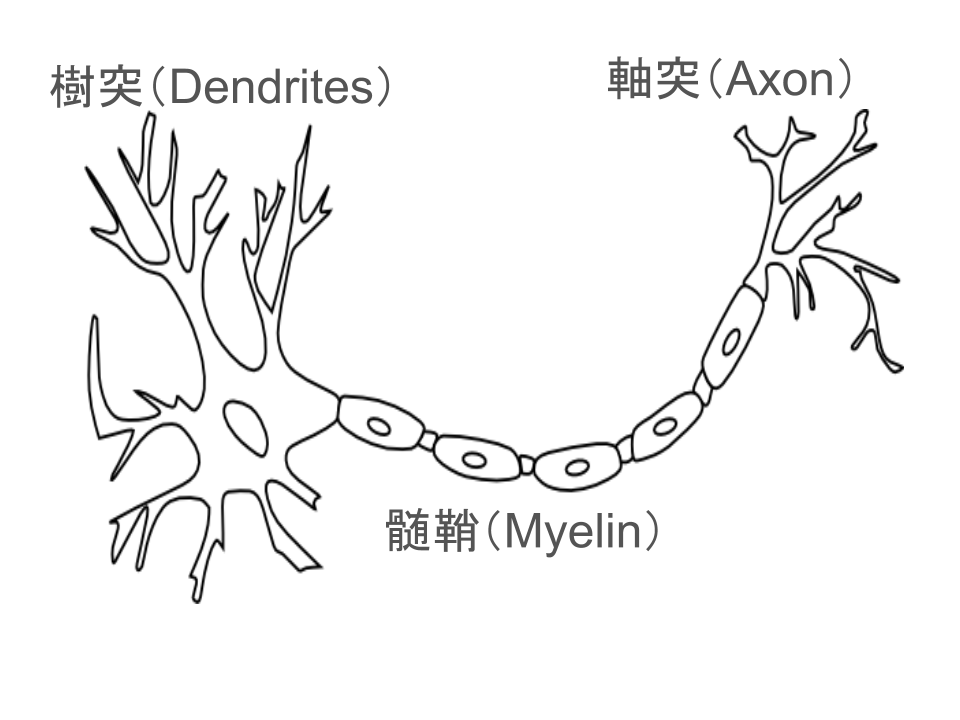
\includegraphics[scale=0.15]{images/chap2_neuron_a.png}\label{fig:chap2_neuron_a}}
\subfloat[][數學上的單顆神經元結構]{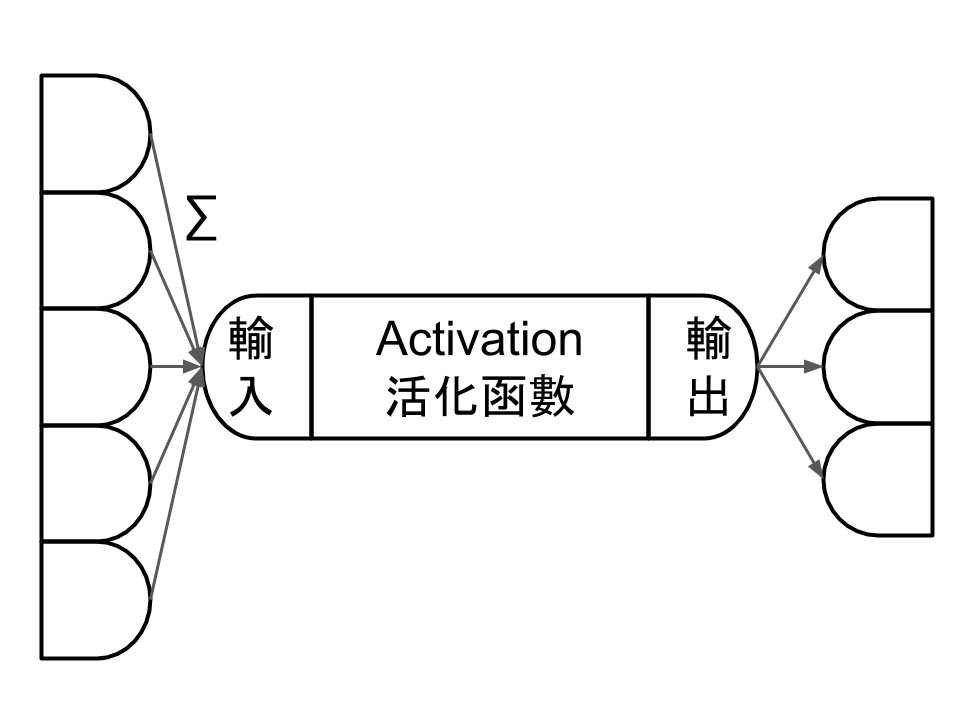
\includegraphics[scale=0.15]{images/chap2_neuron_b.png}\label{fig:chap2_neuron_b}}
\subfloat[][層狀連接的神經網路]{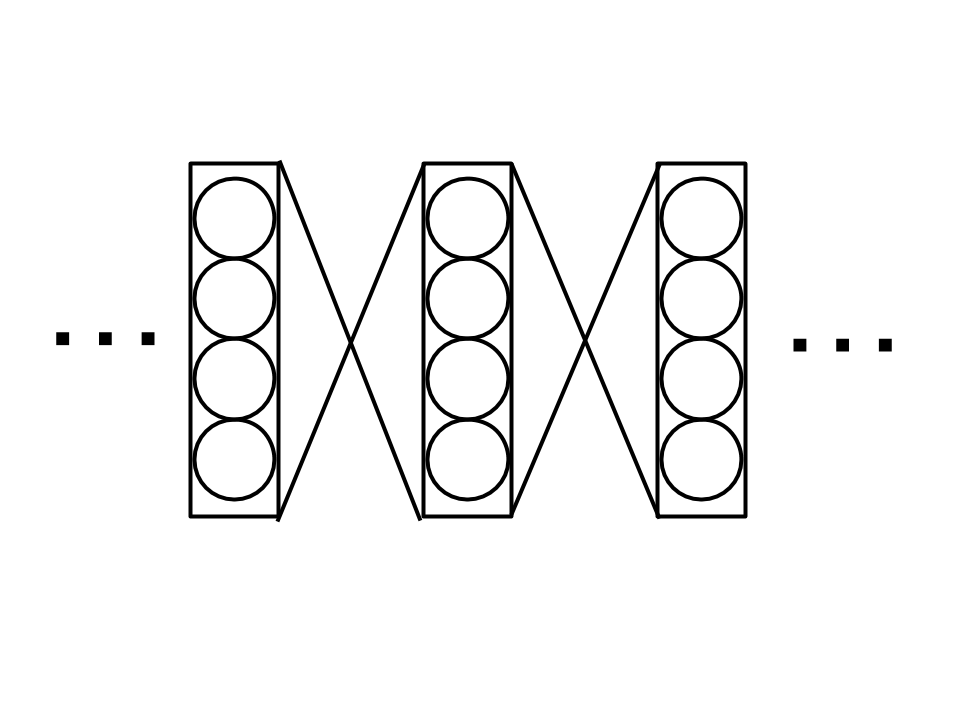
\includegraphics[scale=0.15]{images/chap2_layer.png}\label{fig:chap2_layer}}
\caption{類神經網路的基本架構}
\end{figure}

給定輸入特徵向量$\bold{x} = [x_1 , x_2 , x_3 , x_4 ... , x_D]^T$,與相應的標籤(Label)$\bold{y} = [y_1 , y_2 , y_3 , y_4 ... ,y_C]^T$,我們目標在取得最接近標籤的輸出$\bold{\hat{y}} = [\hat{y}_1 , \hat{y}_2 , \hat{y}_3 ... , \hat{y}_C]^T$。中間隱藏層$\bold{h^{(j)}} = [h^{(j)}_1 , h^{(j)}_2 , h^{(j)}_3 , h^{(j)}_4 ... , h^{(j)}_S]^T$的每一個神經元$h^{(j)}_{i}$都會經由仿射變換(Affine Transform)與非線性活化函數(Nonlinear Activation Function)後輸出。

仿射變換乃計算前一層所有神經元的輸出,進行加權總和(Weighted Summation)和閾值偏移(Threshold bias)。整體的數學式可表示成:
\begin{equation}
h^{(j)}_{i} =
\left\{\begin{matrix}
 \sigma (\sum_{k=1}^{S} w_{ki}^{j}h_{k}^{(j-1)} + b_{i}^{(j)}) & j = 2 , 3 , 4 ... H \\ 
 \sigma (\sum_{k=1}^{D} w_{ki}^{j}x_{k} + b_{i}^{(j)}) & j = 1 
\end{matrix}\right.
\end{equation}

其中$h_i^{(j)}$為第j層隱藏層的第i個神經元輸出;$\sigma$為活化函數;$w_{ki}^{(j)}$與 $b_{i}^{(j)}$分別為神經元突觸權重與活化閾值偏移;S為每一層隱藏層的寬度,代表每層包含的神經元數量;D為輸入層的維度;H為隱藏層的層數。這些都是設計模型的核心參數。

常見的活化函數有兩種,如S型函數(Sigmoid)和整流線性單元(Rectified Linear Unit, ReLU),分別為:
\begin{equation}
sigmoid(x) = \frac{1}{1 + e^{-x}}
\end{equation}
\begin{equation}
ReLU(x) = max( 0 , x )
\end{equation}
深層類神經網路的最後一層亦是仿射變換,但是不再經過活化函數,該層輸出又稱邏輯子(Logits):
\begin{equation}
z_i = \sum_{k=1}^{D} w_{ki}^{(H)}h_{k}^{(H)} + b_{i}^{(H)} 
\end{equation}
當深層類神經網路用作多類別的分類器時,邏輯子會通過軟性最大化轉換(Softmax),變成類似機率分佈的分類輸出:
\begin{equation} \label{eq:softmax}
\hat{y}_i = \frac{e^{z_i}}{\sum_{k=1}^{C}e^{z_k} }
\end{equation}
當深層類神經網路用作多類別的回歸器時,則直接輸出邏輯子的值:
\begin{equation}
\hat{y}_i = z_i 
\end{equation}
深層類神經網路便是藉由每一層權重矩陣$\bold{W}^{(h)} = \{w_{ij}^{(h)}\}$與每一層的偏移閾值$\bold{b}^{(h)}$,將一筆輸入資料$\bold{x}$轉換成輸出資料$\hat{\bold{y}}$的非線性函數$f_{\theta}:\mathbb{R}^D\rightarrow \mathbb{R}^C$,其中$\theta$為DNN的模型參數,也就是上述的權重矩陣與偏移閾值。使用DNN的核心問題,在於如何找到理想的函數$f_{\theta}$,已達到更高的分類準確率或是更少的回歸誤差。
\subsection{訓練方法}
DNN的訓練方式,需要借助損失函數(Loss Function),來模擬DNN與理想函數的量化距離。其訓練的目標可以規化為以下的最佳化問題(Optimization Problem):
\begin{equation}
\min_{\theta}{ \sum_{n=1}^{N}{ {L( \bold{x}_n , \bold{y}_n , \theta)}}}
\end{equation}
其中,$\bold{x}_n$為訓練輸入實例,總共有$N$個。$L(\bold{x}_n , \bold{y}_n, \theta)$為輸入實例$\bold{x}_n$通過模型$\theta$與正確標籤$\bold{y}_n$相比產生的損失。

一般來說,損失函數是模型設計者將真正的期望目標,與類神經網路的輸出結果相比算出來的距離。損失函數的值越大,代表模型的輸出結果與期望目標相差越遠,也因此訓練的目標為最小化損失函數。

以多類別分類器而言,分類器的輸出向量$\hat{\bold{y}}$,會將每一個維度對應到一個分類標籤,總共有$C$種類別。給定的正確標籤$\bold{y}$會公式化為1-hot向量$[0 , 0 , ... , 0 , 1 , 0 ... , 0]^T $,只有正確類別$l$的值是1,其餘為0。訓練此種分類器時,損失函數為交叉熵(Cross Entropy, CE),定義為:
\begin{equation} \label{eq:LCE}
L_{CE}(\bold{x} , \bold{y} , \theta) = KL( \bold{y} || f_{\theta}(\bold{x}) ) = KL(\bold{y} || \hat{\bold{y} }) = \sum_{i = 1}^{C} y_i \log{ \frac{y_i}{\hat{y}_i} } = - \log \hat{y}_{l} 
\end{equation}

其中$KL(p||q)$代表的是克雷散度(Kullback–Leibler Divergence),用以衡量兩組機率分佈的距離,值越大則代表兩組分佈越不相似。$L_{CE}$計算了分類器的正確標籤$\bold{y}$與通過模型參數後的預測向量$\hat{\bold{y}}$的克雷散度,但由於$C$種正確標籤中,只有一個類別$l$的值為1,也因此$L_{CE}$可以簡化成公式\ref{eq:LCE}最右邊的簡單型態,最小化正確分類標籤的負對數可能性(Negative Log Likelihood, NLL)。

以多類別回歸器而言,則更廣義地希望將回歸器的輸出向量$\hat{\bold{y}}$與目標向量$\bold{y}$的距離拉近。訓練此種分類器時,距離的衡量通常為均方差(Mean Square Error, MSE),定義為:
\begin{equation}
L_{MSE}(\bold{x} , \bold{y} , \theta) = || \bold{y} - f_{\theta}(\bold{x}) ||_2 = || \bold{y} - \hat{\bold{y}} ||_2 = \sum_{i = 1}^{C} ( y_i - \hat{y}_i )^2 
\end{equation}

當模型設計者決定好適當的損失函數後,下一個問題便是選擇解決最佳化問題的演算法。理想上,理想參數應能夠最小化損失函數:
\begin{equation}
\theta^* = \arg\min_{\theta}{ \sum_{n=1}^{N}{ {L( \bold{x}_n , \bold{y}_n , \theta)}}}
\end{equation}

但是因為DNN中間飽含非線性活化函數的緣故,最小化損失函數通常沒有方便可得的解析解(Analytical Solution),或稱封閉解(Close-form Solution)。實務上,通常採用迭代式(Iterative)演算法,給定一個參數起點,一步一步減少損失函數。
最簡單的迭代式最佳化演算法為統計式梯度降低(Stochastic Gradient Descent)演算法,給定某一組參數$\theta$,損失函數沿著該參數上的梯度方向更新,下降的速度最快,可表達成:
\begin{equation}
\theta_{k+1} \leftarrow \theta_k - \eta \Delta \theta_{k} 
\end{equation}
\begin{equation}
\Delta \theta_{k} = \frac{\partial L}{\partial \theta} \biggr|_{\theta = \theta_k}
\end{equation}
其中$\eta$為學習比率(Learning rate),調控最佳化的速度與精細度,$k$為更新的階段,隨著$k$的增加,可期望損失函數的值越來越小,模型越接近理想模型。

然而梯度的計算牽扯到函數的一次微分,對於雜訊的反應較不穩健,訓練上不穩定。更進階的訓練方式包含了慣量(Momentum),使得每次SGD更新的時候,包含了前次更新的梯度方向,可表達為:
\begin{equation}
\Delta \theta_{k} =  \mu \Delta \theta_{k-1} + \frac{\partial L}{\partial \theta} \biggr|_{\theta = \theta_k}
\end{equation}
其中$\mu$為慣量係數,用以調控慣量的比例。

在使用SGD訓練DNN的時候,通常是使用反向傳播(Back Propagation)演算法,在DNN完成順向預測(Forward Prediction)計算出$\hat{\bold{y}}$後,會先得到最後一層參數的梯度值,再根據鏈鎖律(Chain-rule),將梯度反向傳播回輸入層,取得每一層的參數的梯度值,從而完成一次更新。
使用最佳化演算法訓練DNN的時候,沒有任何方法可以保證損失函數是下凹(Convex)的。在損失函數下降的過程中,並不保證會下降到最佳解(Global Optimum)上,很有可能會停在局部最佳解(Optimal, or Local Optimum)上。因此在訓練之初通常使用隨機初始化,並且擴增模型的隨機性,以避免掉落到結果較差的局部最佳解上。

\begin{figure}
\centering
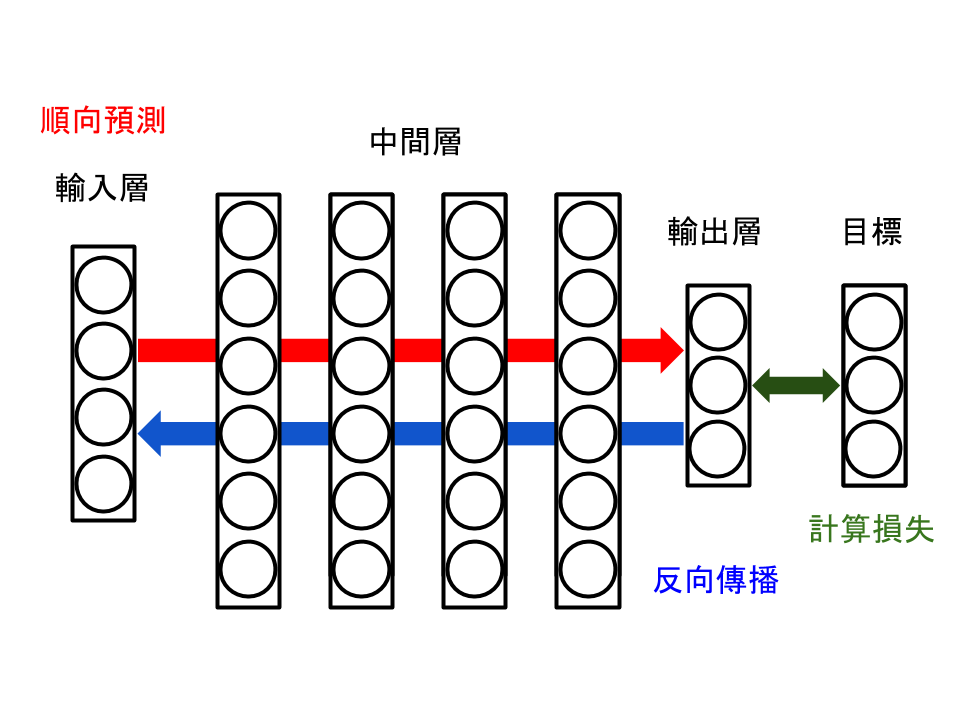
\includegraphics[scale=0.35]{images/chap2_dnn.png}
\caption{深層類神經網路訓練示意圖}
\label{fig:chap2_dnn}
\end{figure}

\subsection{丟棄演算法}
所有的機器學習模型,都會陷入過度適應(Overfitting)的情況。發生過度適應時,模型能夠在訓練集上達到很好的表現,卻在測試集上表現得越來越差。這時候模型的概括化的能力正逐漸下降,而是單純記憶輸入資料的規律與數字,無法學習到真正幫助辨識學習的本質。
最常見避免過度適應的方法,就是使用控制調適(Regularization)。使用控制調適,可以縮減模型複雜度,卻不會縮減模型強度,如在損失函數上額外添加控制參數大小的控制子。針對DNN,辛氏提出了丟棄演算法(Dropout):順向預測時,每個神經元會有$p$的機率直接關閉,無法活化,使得輸出值為$0$,如圖\ref{fig:chap2_dropout_b}與圖\ref{fig:chap2_dropout_c}。藉由隨機丟棄,可以強迫模型中的各種參數自力更生,而不是相互適應,強迫模型學到更概括化的能力。


\begin{figure}
\centering
\subfloat[][未經丟棄的DNN]{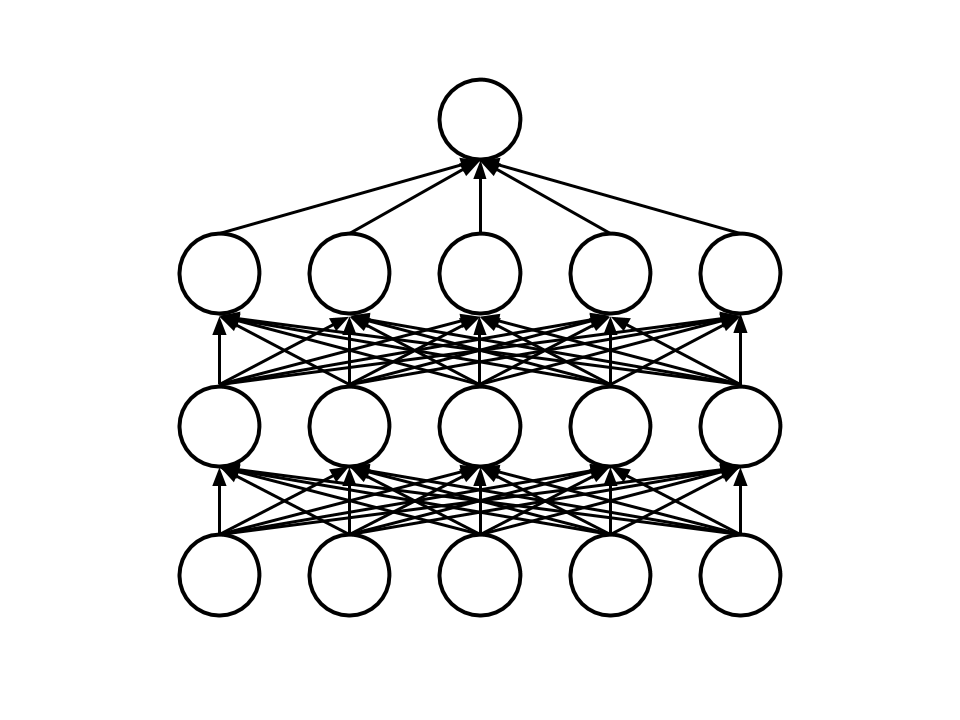
\includegraphics[scale=0.15]{images/chap2_dropout_a.png}\label{fig:chap2_dropout_a}}
\subfloat[][隨機丟棄部份神經元的DNN]{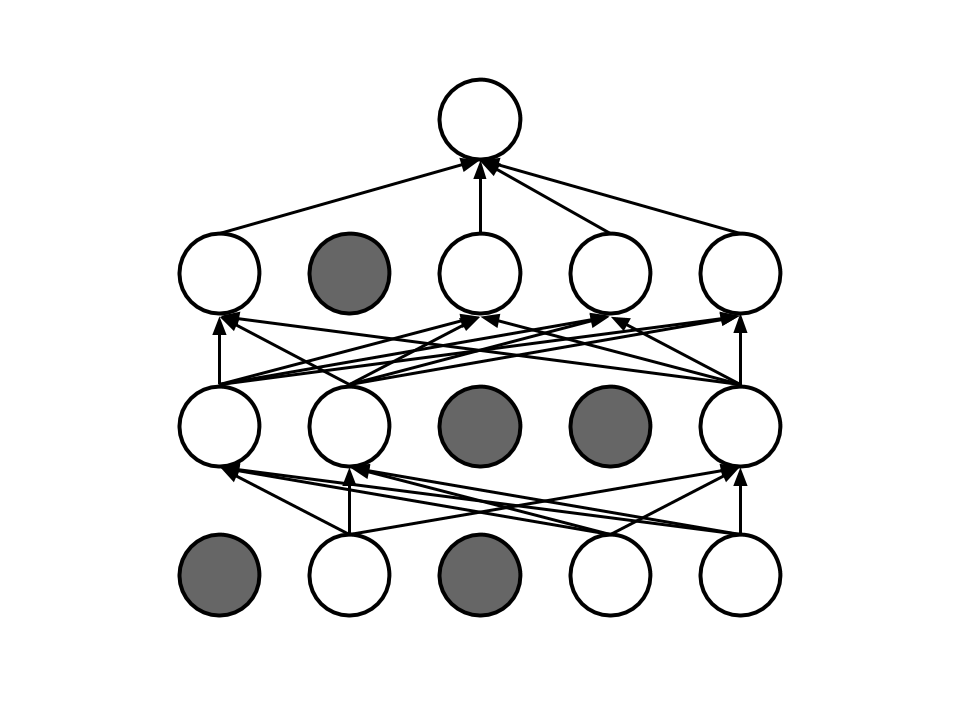
\includegraphics[scale=0.15]{images/chap2_dropout_b.png}\label{fig:chap2_dropout_b}}
\subfloat[][隨機丟棄部份神經元的DNN]{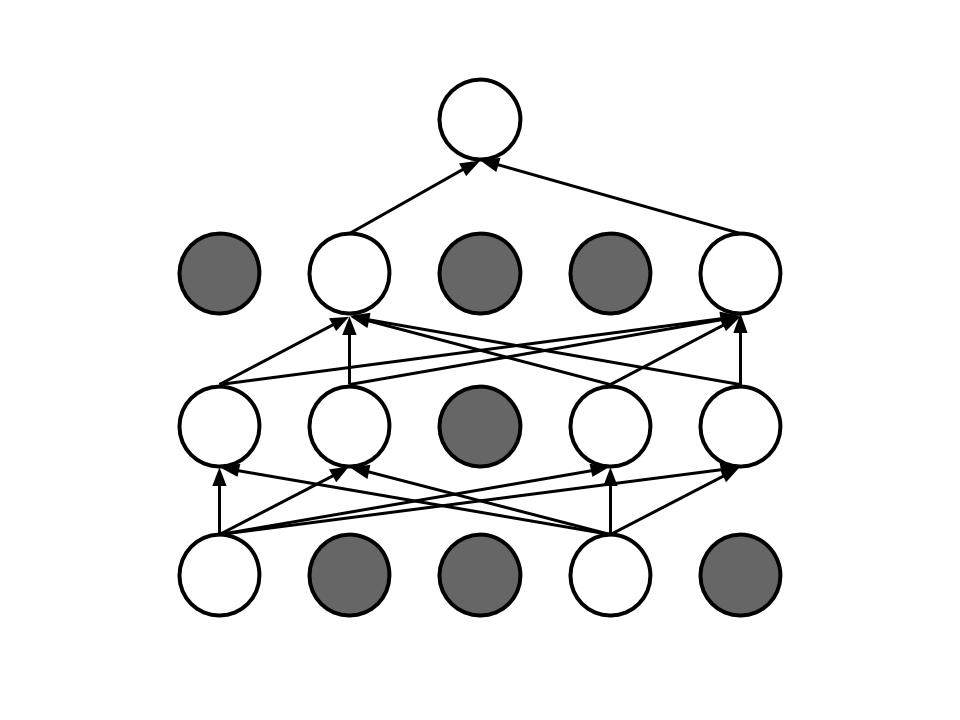
\includegraphics[scale=0.15]{images/chap2_dropout_c.png}\label{fig:chap2_dropout_c}}
\caption{丟棄演算法示意圖。其中(b)與(c)是兩種不同的丟棄配置,因為隨機性而有了多樣化,分別是較小的模型,但整合成一個比(a)來得強大的整合模型。}
\end{figure}

丟棄演算法同時也可以視為隨機整合(Random Ensemble)模型。整合模型(Ensemble Model)在機器學習領域已經被證明是非常強大的模型,藉由多個模型的多樣性(Diversity)各司其職,提昇模型強度。類比在丟棄演算法中,根據不同的丟棄情況,有不同的神經元組合互相整合而成。隨機性造就了多樣性,又同時控制調適,使得模型更不容易過度適應。
\section{全球音素語料庫(GlobalPhone Corpus)}
\subsection{語料介紹}
全球音素語料庫(GlobalPhone Corpus, GP)是德國卡斯魯爾大學(Karlsrusher University, 現在卡斯魯爾理工學院前身)的譚雅.修姿女士(Tanja Schultz)所主持、設計與收集的多語言語料庫,專門設計給語音辨識系統發展與研究使用。語料庫內含15種語言,每種語言也有80位以上的語者變化,使得語料庫總計有300小時以上的聲音檔,1500位以上的在地成人語者聲音資料庫。不同語言間的錄製環境、設計準則皆一致,唯有語言和語者的差異,以方便進行跨語言的系統設計與實驗比較。

GP發展之初,是為了研究獨立於語言之間的全球音素集(Global Phone Set),以輔助相依於不同語言的的辨識系統,從其全球音素之命名可見一斑。語言學家對於多語言辨識系統具有高度興趣,需要品質較好、設計準則一致又富含多樣化語言的語料庫,這樣的需求顯然催生了GP。然而世界語言已經超過4500種,GP在挑選語言上亦費了一番功夫。為了挑選最能代表世界語言的組合,GP至少考量了:
\begin{itemize}
\itemsep -2pt 
 \item 語者數量
 \item 語者政治跟經濟環境多樣性
 \item 地理範圍(然非洲因無穩定經濟體系,語料收集困難,語系亦複雜多變,故無考慮非洲)
 \item 語言包含的音素範圍
 \item 語系和語形分佈。
\end{itemize}
GP先於當時的國內外報章雜誌中蒐集政經相關文字,由指定語者唸出文字錄製而成,是為閱讀型語音(Read Speech)。所有的語音都在一兩年內錄製完成,確保每個語言之間共通名字(如政治家、都市、公司)的一致性。這些錄音檔都經過人工的二次確認,包含斷句、發音錯誤等等。除了聲音所對應的文字以外,亦額外收集大量的文字資料。這些資料並不額外錄音,僅供訓練語言模型。


本論文選擇了GP四個印歐語系語言,分別為西斯拉夫語支的捷克語(Czech, CZ)、西德語支的德語(German, GE)、西伊比利亞語支的西班牙文(Spanish, SP)、和高盧羅曼語支的法文(French, FR)。這四個語言的基本資料如附錄。
\subsection{國際音標(International Phonetic Alphabet, IPA)}
國際音標是語言學家為了更有效率表達世界上各種語音而設計的一套符號規則。最早由國際語音學學會(International Phonetic Association)所建,而後修改擴充,以清楚描述世界上任何人類語音的聲音。

針對任一語言,國際語音學學會會針對其中的每一個可鑑別音(Distinctive Sound),進行音素轉寫(Phonetic Transcription),對應到國際音標上的一種獨立符號。即便物理上兩者呈現不同的聲音,但如果在該語音母語人士人耳中無法鑑別,則必須被標記為同一種音素(Phone)。因此,一種語言通常只會用到部份的國際音標。

國際音標中最常使用的通常為母音(Vowel)與子音(Consonant)的部份,合稱肺部氣流音(Pulmonic)。母音在國際音標中,以母音四邊型(Vowel Quadrilateral)的方式呈現,如圖\ref{fig:vowel};子音則為一張藉由發音方式以及發音位置交錯整理而成的表格,如圖\ref{fig:consonant}。

\begin{figure}
\centering
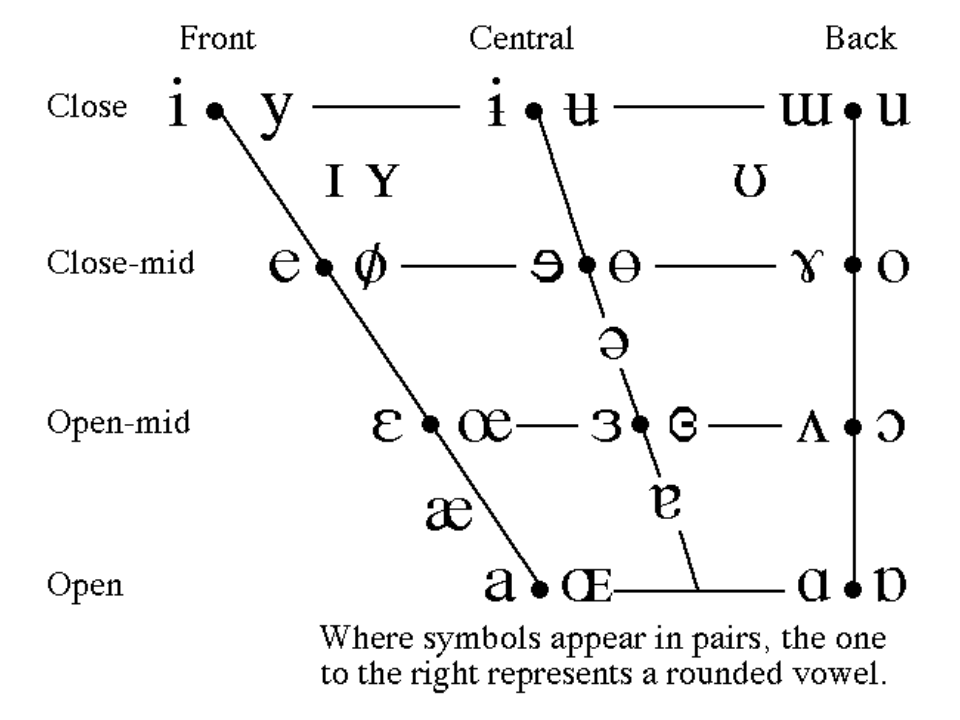
\includegraphics[scale=0.4]{images/chap2_vowel_quadrilateral.png}
\caption{母音四邊形}
\label{fig:vowel}
\end{figure}

\begin{figure}
\centering
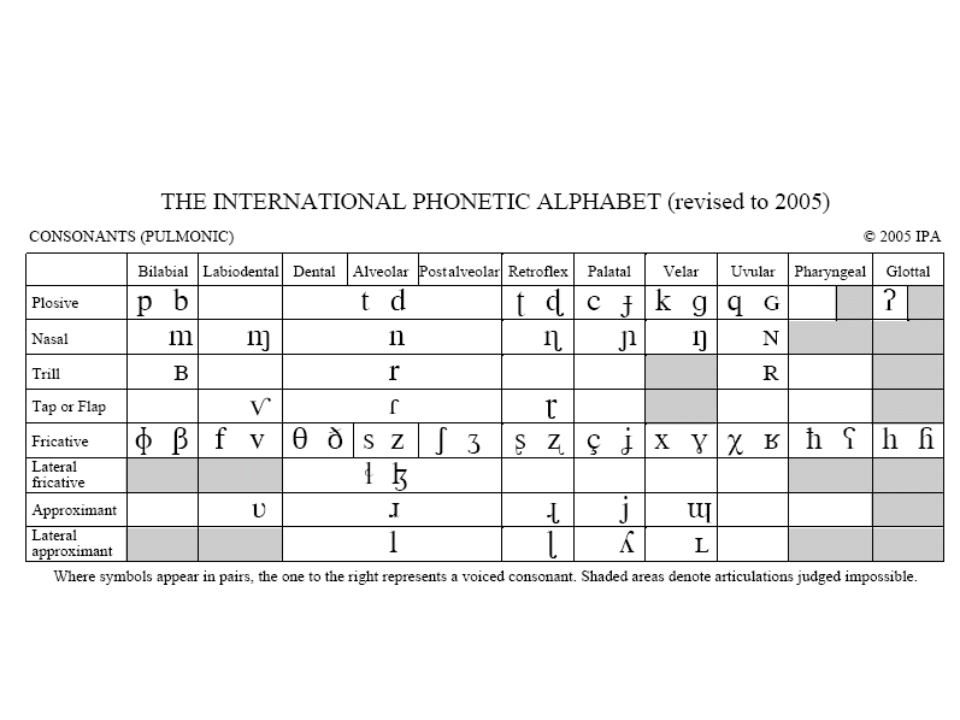
\includegraphics[scale=0.4]{images/chap2_consonant.png}
\caption{子音表}
\label{fig:consonant}
\end{figure}
母音四邊形類比於人類口腔,每一點代表發音時,舌頭在口腔中的接觸位置。左右代表口腔前後,上下亦然。同一位置上如有兩種音素,右音素為圓唇音(Rounded),一如其名,發音時須圓唇。

子音表格中,左邊根據不同發音方式分類,上邊根據不同發音接觸位置分類。同一位置上如有兩種音素,右音素為聲帶靠近時發出的濁音(Voiced),左音素則為聲帶遠離時發出的清音(Unvoiced)。有些格子為灰色,代表人類不可能發出的發音組合。

一般而言,子音與母音已經能夠廣義地涵蓋所有發音單位。然各語言有其特色,往往需要額外地在廣義轉寫符號上標記各種程度的細節,形成讀音符號(Diacritic)。本論文所選的四種語言,除了其原生的音素以外,亦標記了各個音素對應的國際音標表於附錄。

\section{多語言語音辨識系統}
多語言語音辨識系統的發展,有各種不同的情景,相關的研究亦有不同的靈感、切入點以及評估方式:
\subsection{語言混合(Code-Mixing)}
有些地區的人民,可能因為科技發展、地緣關係的因素,同時熟稔兩種以上的語言,其熟稔程度除了單純的句子交錯、名詞抽換之外,甚至有可能文法參雜,借用別的語言的句式。這些語言混合(Code-Mixing, CM)的核心問題,在於如何準確找到語者切換不同語言時的切換點(Code-Switching Point, CS Point)。如圖\ref{fig:chap2_cs}。

語言混合的例子,隨著時代變遷越來越明顯,如:
\begin{itemize}
\itemsep -2pt
\item 歐盟(European Union, EU)裡每個成員都具備至少三種語言的隨時切換能力,常會有一個人以德文發問、另一人以西文回答、第三人用德文混法文補充。
\item 亞洲的教育體系往往保留原文的發音與字詞,如在中文的文法裡中加入英文的專有名詞。
\end{itemize}
語言混合的問題,通常會將語言分為基質語言(Matrix Language)與嵌入語言(Embedded Language),這樣的分類主要根據混合比例。基質語言通常是語者的原生語言,決定該句子的文法句式和主要發音音素。嵌入語言則為客串,若基質語言無法呈現某些關鍵意涵時,語者可能轉而使用嵌入語言表達。然基質語言和嵌入語言的比例不均,在訓練語音辨識系統時,造成系統偏好資料量較多的基質語言,而無法成功辨識資料量較少的嵌入語言。

為了解決資料量不足的問題,可以將基質語言和嵌入語言中近似的發音單位合併訓練。合併單位可能從較高層級的音素層級、越發細緻到更底層的三連音態(Triphone state, or Senone)層級,如圖\ref{fig:chap2_merge}。
\begin{figure}
\centering
\subfloat[][語言混合資料示例,黃線為語言切換點]{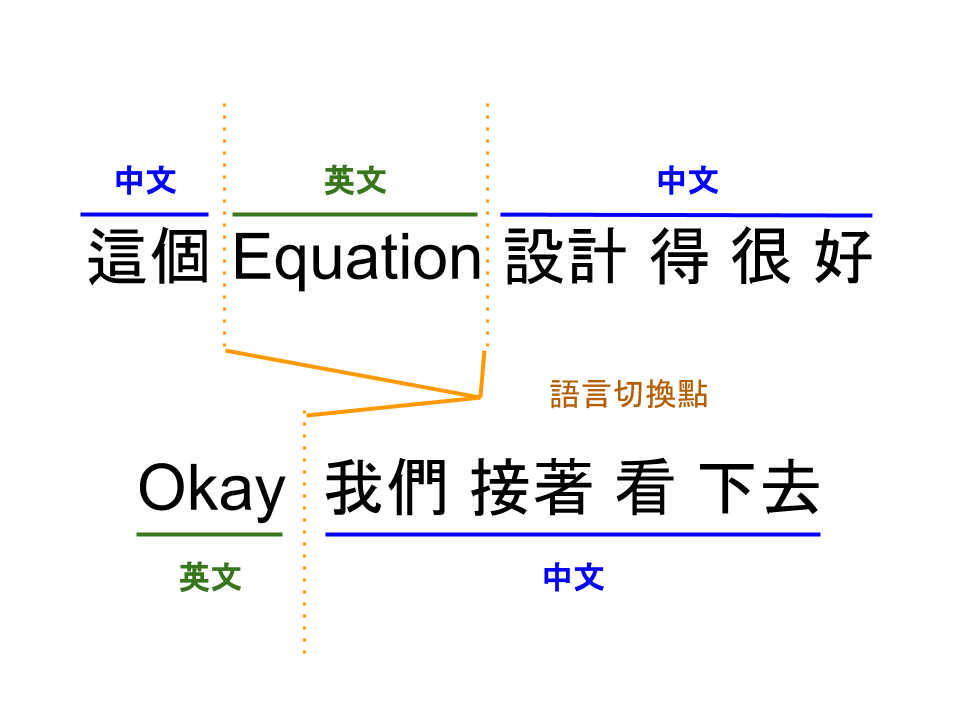
\includegraphics[scale=0.25]{images/chap2_cs.png}\label{fig:chap2_cs}}
\subfloat[][三連音態合併的深層類神經網路訓練]{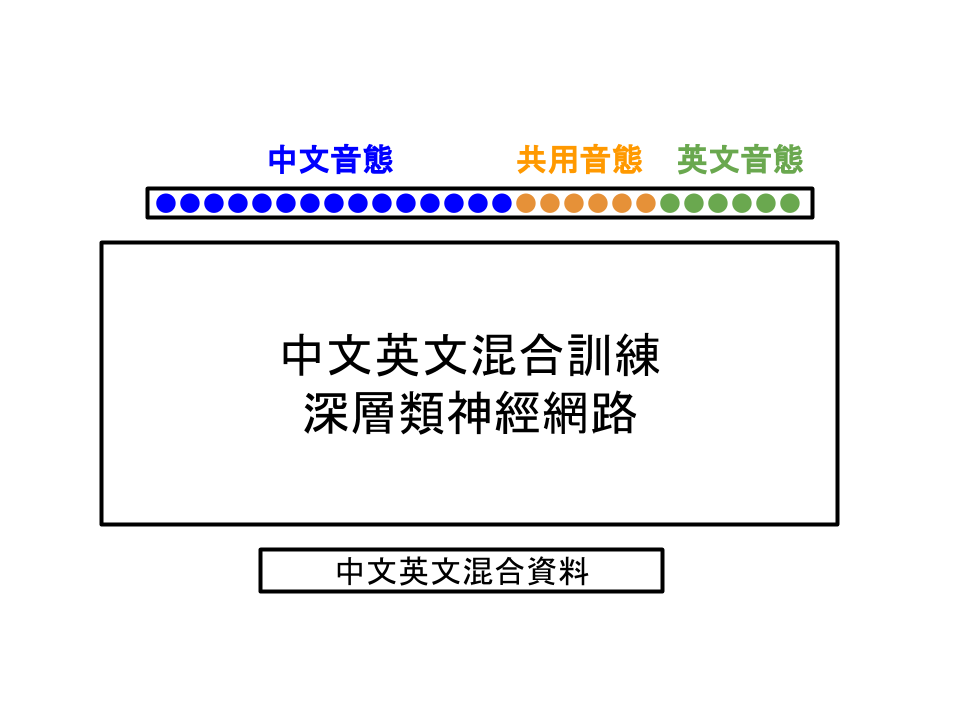
\includegraphics[scale=0.25]{images/chap2_merge.png}\label{fig:chap2_merge}}
\caption{以中文混合英文的語言混合問題與模型訓練方法。}
\end{figure}
%因應比例不同,亦可以先訓練嵌入語言偵測器,當偵測器發現時嵌入語言時,將嵌入語言的事後機率拉高,形成模糊化事後機率特徵(Blurred Posteriorgram Features, BPFs)。

在評估語言混合問題時,除了兩種語言的結果都必須分別分析之外,因為嵌入語言的數量較少,討論時往往深入探討嵌入語言的辨識率。


\subsection{跨語言轉移學習(Crosslingual Transfer Learning)}
跨語言轉移學習是借助豐富大量的來源語言(Source Languages),以幫助資源稀少(Low-resourced)的目標語言(Target Language)訓練語音辨識系統。當資料量過少的時候,一般的機器學習方法就容易陷入瓶頸,遑論亟需資料量的深度學習。
例如非洲、東亞戰亂地區的語言。這些語言本身收集困難,又因為軍事政治環境的關係,有語音辨識或是關鍵字擷取(Keyterm Extraction)的需求。軍方有可能採集少量的該地聲音作為目標語言。相比之下,GP的資料量非常豐富,也非常乾淨,與資源稀少的語言相當不匹配。

語言間或多或少有共通的聲音特色,常見的轉移學習便是以大量豐富資料前置訓練(Pretraining)一個來源語言的語音辨識系統,再以目標語言的少量資料微調(Fine-tune)成目標語言的語音辨識系統,如圖\ref{fig:chap2_cross}。

\begin{figure}
\centering
\subfloat[][以來源語言訓練]{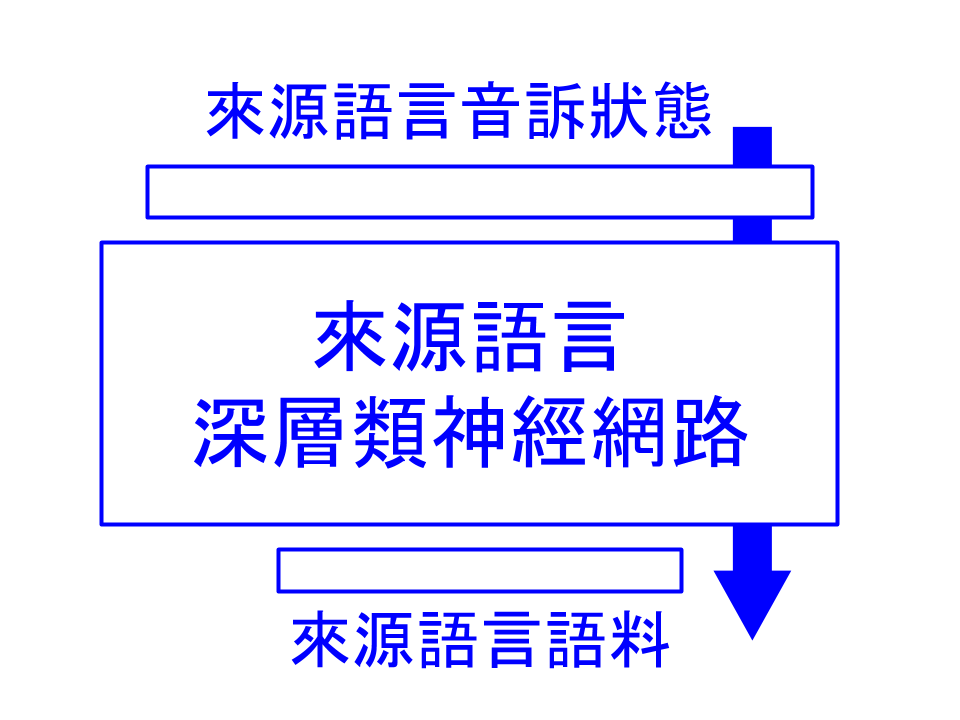
\includegraphics[scale=0.15]{images/chap2_cross_source.png}\label{fig:chap2_cross_source}}
\subfloat[][以目標語言微調]{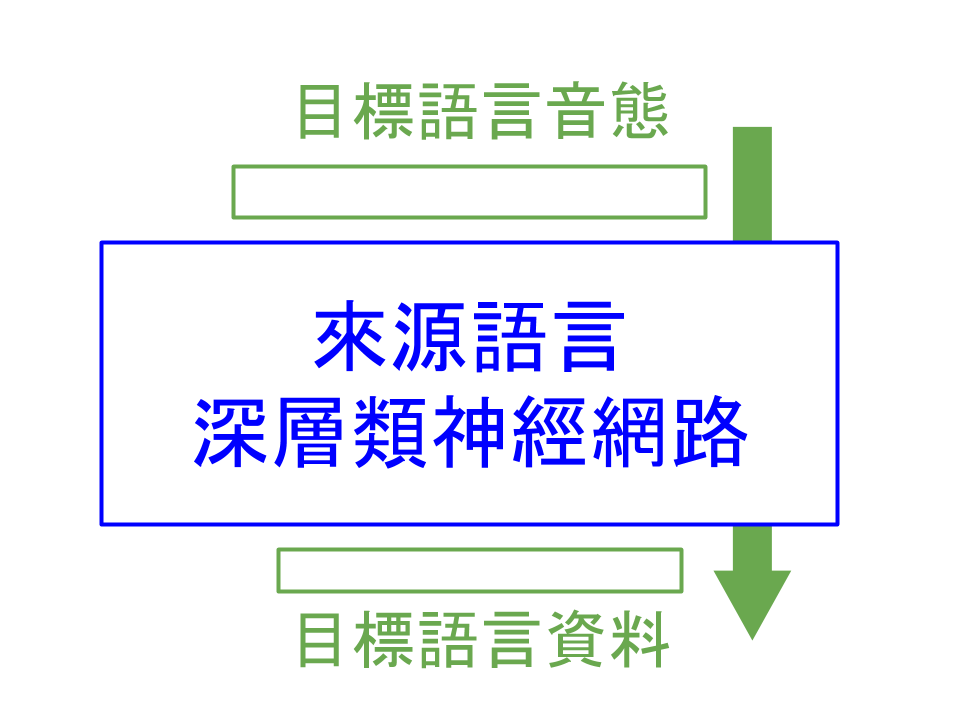
\includegraphics[scale=0.15]{images/chap2_cross_target.png}\label{fig:chap2_cross_target}}
\subfloat[][微調後模型同時包含兩者資訊]{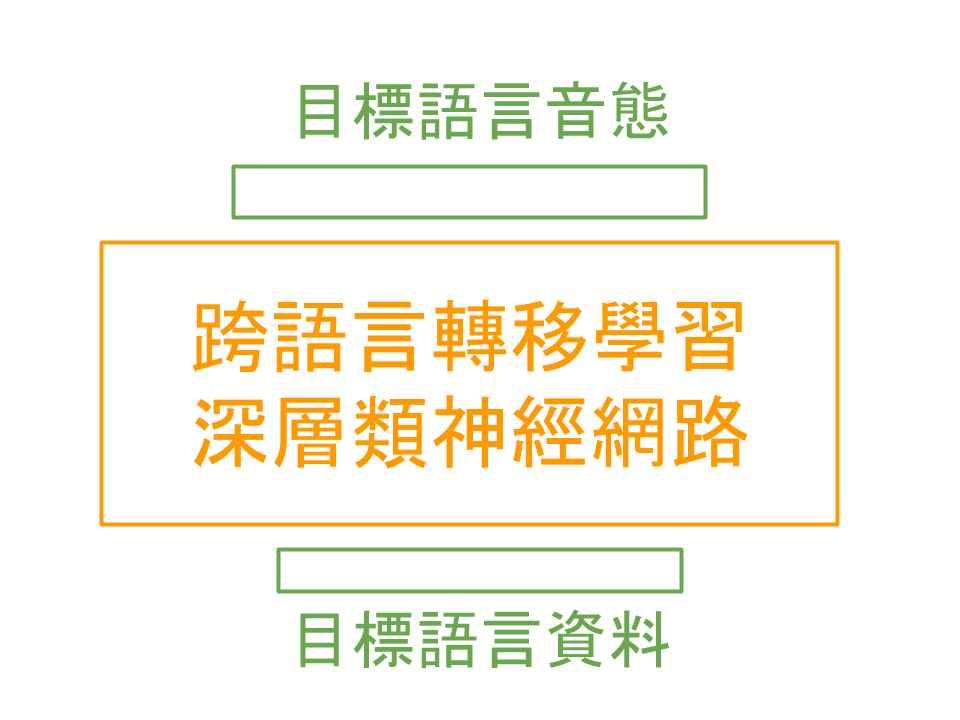
\includegraphics[scale=0.15]{images/chap2_cross_finetune.png}\label{fig:chap2_cross_finetune}}
\caption{訓練跨語言轉移學習類神經網路,由左至右依序訓練,箭頭則是訓練時從輸出反向傳播至輸入的方向。}
\label{fig:chap2_cross}
\end{figure}


\subsection{多語言共享學習(Multilingual Sharing)}
結合上述的情景,多語言語音辨識系統的關鍵,便是能否在多如繁星的各種語言中,找尋共通的資訊,彼此輔助學習。一來減少對單一語言的資料量依賴性,二來可以提供更多語言的語音辨識系統,如圖\ref{fig:chap2_multilingual}。這包含了許多種不同層級的共享,像是語言混合問題中提到的發音單位共享,或是跨語言轉移學習中提到的模型微調。

但這個問題並不像語言混合一樣針對嵌入語言,也不似跨語言轉移學習問題中一樣針對目標語言。多語言共享學習希望能找出不同語言中的共享精華,例如全球音素集,或是更細緻的全球音態集(Global Senone Set),因而對待每個語言的比重平等,旨在希望不同語言間的資訊可以互惠,而不是單方面的施與受。在評估表現時,須特別注意多個語言表現的整體性,以免顧此失彼。

\begin{figure}
\centering
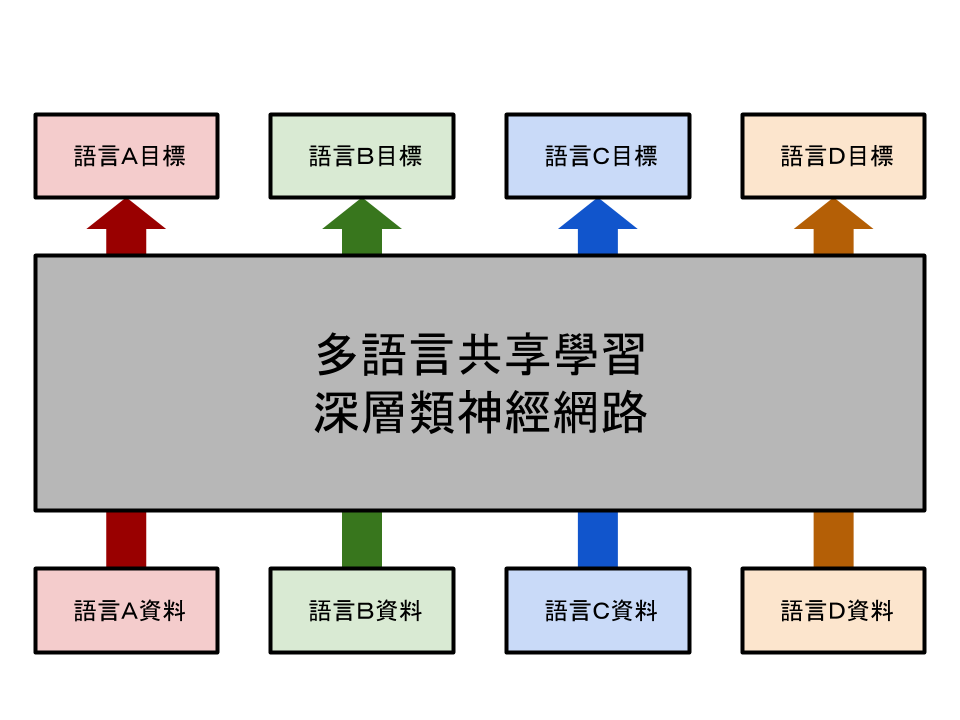
\includegraphics[scale=0.4]{images/chap2_multilingual}
\caption{多語言共享學習,四個語言各自獨立評估卻又相輔相成,互相學習。}
\label{fig:chap2_multilingual}
\end{figure}
